\documentclass[12pt, a4paper]{report}
\usepackage[pdftex]{graphicx} %for embedding images
\graphicspath{ {./img/} } %the path to the images
\usepackage[,italian, english]{babel}
\usepackage{url} %for proper url entries
% \usepackage[bookmarks, colorlinks=false, pdfborder={0 0 0}, pdftitle={<pdf title here>}, pdfauthor={<author's name here>}, pdfsubject={<subject here>}, pdfkeywords={<keywords here>}]{hyperref} %for creating links in the pdf version and other additional pdf attributes, no effect on the printed document
%\usepackage[final]{pdfpages} %for embedding another pdf, remove if not required

\begin{document}
\renewcommand\bibname{References} %Renames "Bibliography" to "References" on ref page


\begin{titlepage}

\begin{center}

\Large \textbf {Programmazione Concorrente e Distribuita - Assigment 03}\\%\\[0.5in]
\vspace{1em}%
\vfill
Leonardo Randacio


Filippo Gurioli


Andrea Biagini
\vspace{1em}
\vfill
{\bf Università di Bologna \\ Scienze e Ingegneria Informatiche}\\[0.5in]

       
\vfill
\today

\end{center}

\end{titlepage}


\tableofcontents
\listoffigures

\newpage
\pagenumbering{arabic} %reset numbering to normal for the main content

\chapter{Analysis}
The goal is to create a concurrent agent-based simulation.

An agent-based simulation or model is a computational modeling
 technique used to simulate complex systems by representing individual
 entities, known as agents, and their interactions within an environment.
 The goal of the simulation is to observe the evolution of the states of the
 environment and the agents in each discrete step.

Agents beheviour for a single step can be described in 3 phases:
\begin{itemize}
   \item sense phase: the agent acquires data from the environment
   \item decide phase: the agent determines the next action
   \item act phase: the action determined is executed on the environment
\end{itemize}

\section{Task Decomposition}
Each agent's step can compose a single task, which can be divided into 3 subtasks,
 one for each phase of the step. 

This means that for a given step there will be 3 tasks:
\begin{itemize}
    \item sense
    \item decide
    \item act
\end{itemize}

The total number of tasks for a given step is 3 * nAgents
 where nAgents is the number of agents.

\section{Data Decomposition}
The environment can be subdevided in agent's states which
 means the data can be divided in nAgents indipendent states.

\section{Dependency Analysis}
The sense and decide tasks can be joined in a single
 sense-decide task as the sense task only quearies the
 environment and the decide task updates the next action
 to be performed for a given agent. Since the decide phase
 only sets the next action for a given agent and for a
 given step every agent's next action will be set only
 by one decide task, the sense-decide tasks can be executed
 in a concurrent manner.

%The act task must be serialized as the definition imposes that
% a simulation must give the same results indipendently from it
% being implementes sequentialy or concurrently. This means that
% act tasks must be executed in an orderly manner.
The act tasks in a given step can be parallelised between each other, but
 must be executed after the sense-decide task.

The steps of the simulation must be serialized.

\chapter{Design}
Using agenda parallelism we design the system around an agenda
 composed by the various tasks, which were defined earlier. Every
 step in the simulation imposes a mandatory syncronization.

\section{Architecture}
The master-worker architecture is a natural implementation of
 agenda parallelism, using a bag of works. The bag of works is
 implemented as a bounded buffer.

The environment is implemented as a readers-writers monitor, which
 lets threads read from the environment in a parallel manner, but imposes
 that no writing can be executed concurrently with other writing or reading.

2 Latches are used for syncronization between master and workers.

\section{Visual Formalisms}

\begin{figure}
    \centering
    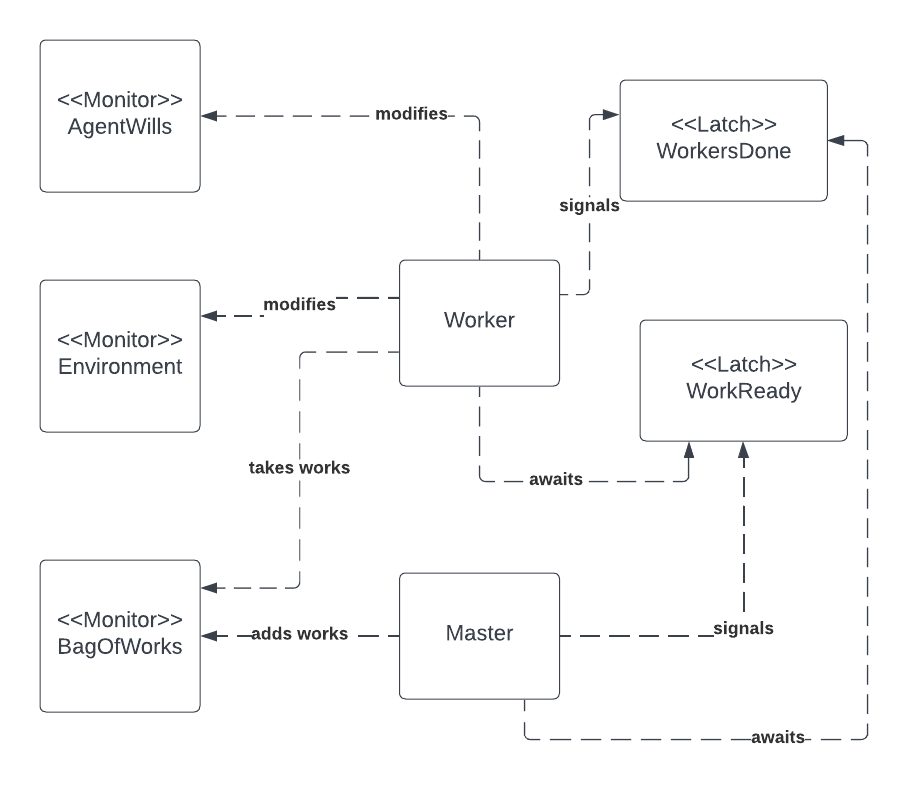
\includegraphics{UML1.png}
    \caption{UML diagram showing relationships between monitors, active components and syncronization components}
\end{figure}

\begin{figure}
    \centering
    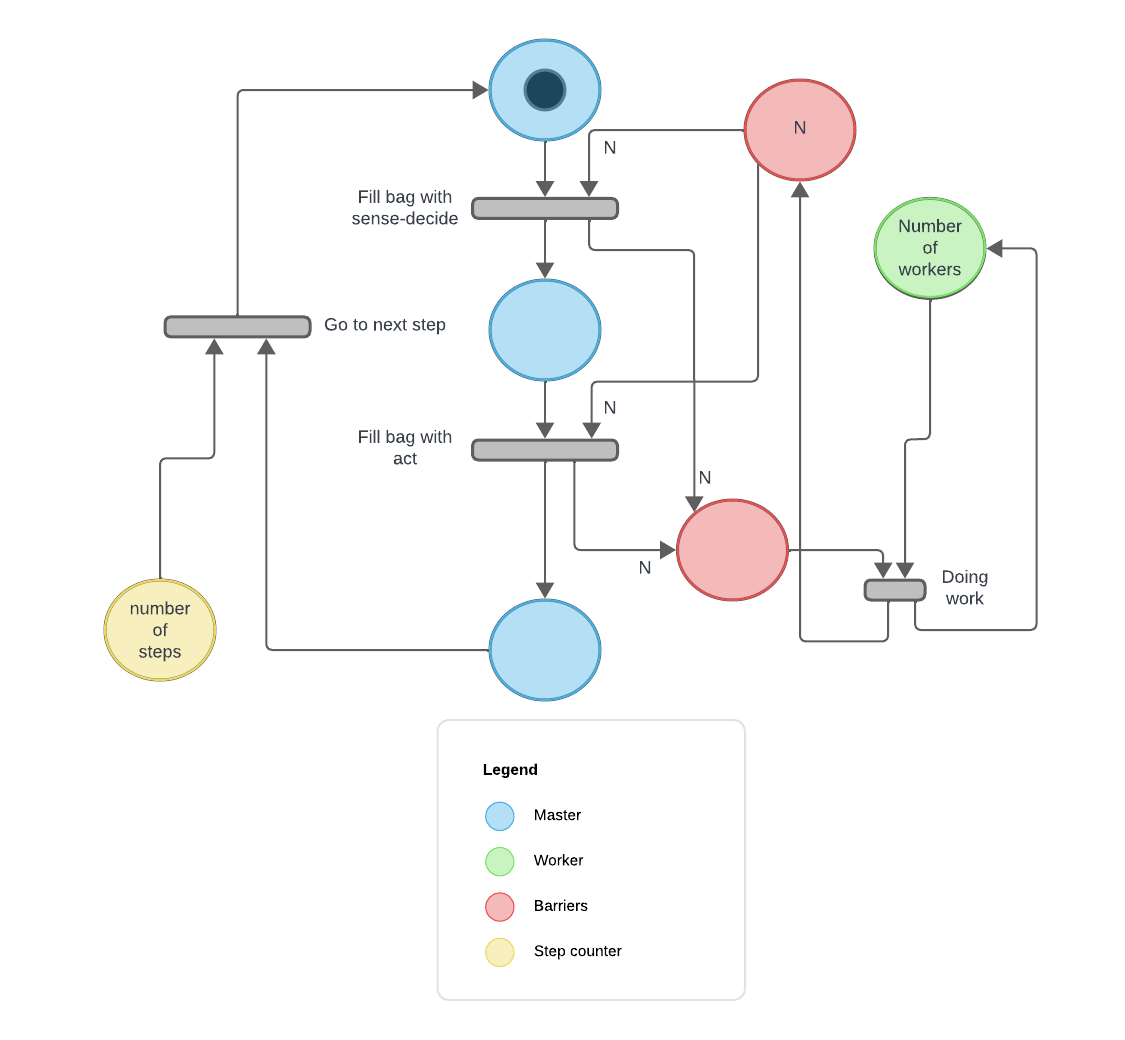
\includegraphics{PetriNetColored.png}
    \caption{Petri net diagram showing the beheviour of the master and workers threads. N is the number of agents in the simulation. The master beheviour is rappresented by 4 places and 4 transitions. The worker is rappresented by one place and one transition. A place containing a token for every step of the simulation regulates the number of steps. Two places rappresent the number of tasks in the bag and the number of tasks finished, regulate the syncronization between master and workers}
\end{figure}

\chapter{Implementation}

\section{Deadlock Problems Encountered}
During implementation some deadlock problems arised.

\subsection{Worker Initialization}
A certain state of the system caused some workers to be left behind.
 After being initialized a worker could start waiting on the \texttt{workReady} latch after
 the master started a step. This caused a deadlock as the worker waited indefinitely
 for the master to signal that the bag was full and the master waited indefinitely for
 all the workers to signal they where ready to recieve other work.

This was solved by having the master wait on the \texttt{workersReady} latch after initializing
 the workers. This way, when the first step of the simulation started, all workers where
 ready to start, making sure no worker was left behind.

\subsection{Check and Act}
A certain state of the system caused two workers to access the bag of tasks even though
 only one work remained in it. This meant that one of the workers would complete the task
 while the other one would await on the notEmpty condition of the bag of tasks. Since the
 master waits for all the workers to notify that they are ready for the next tasks, it would
 never fill the bag with new tasks, waiting indefenetly for the awaiting worker to notify
 it was ready to continue. This is a classic check and act problem.
 
This was solved by making the buffer return an \texttt{Optional} istead of a \texttt{Runnable}. The worker
 now receives an empty \texttt{Optional} from the bag if it was empty, instead of awaiting for the
 bag to be filled again. The notEmpty condition was removed from the bag of works monitor.

\subsection{True Syncronization}
The fact that a worker executed the \texttt{countDownLatch()} on the workers
 ready latch and the \texttt{await()} on the work ready latch in a non atomic way,
 the master could execute the \texttt{countDownLatch()} on the work ready latch, signaling
 to the workers that the bag was full of new works, before
 all the workers where awaiting on it. This would make it so that the master would
 wait for the workers to signal that they had executed all the works available but
 some workers would wait for the master to signal that the bag was full.

This was solved by eliminating the \texttt{workReady} latch, exchanging it for a condition
 of the bag of tasks: notEmpty. This means that workers no longer wait on a latch
 but wait directly on the notEmpty condition inside the bag of tasks. Before blocking
 a worker the bag of task executes the \texttt{countDownLatch()} on the workers ready latch,
 telling the master that a worker has paused. The master is then signaled that all
 workers are paused through the workers ready latch and as soon as a new task is added
 to the bag by the master a worker is woken to resume it's working loop.

\section{Components}
The master and worker threads are the active components. The bag of tasks, the environment, the agent wills and the workers ready
 latch are all passive components, implemented as monitors

\section{Source Code Organization}
The basic simulation implementation has been extended with the GUI implementation

The GUI source code is comprised of only one class: simtrafficexamplesconcurrent/RoadSimView.java

The class simtrafficexamplesconcurrent/RoadSimView.java prints information of the simulation on the terminal

The src is organized in the following packages:
\begin{itemize}
    \item masterworker: containing classes for the master worker pattern implementation
    \item simengineconcurrent: abstract classes for the simulation framework
    \item simtrafficbaseconcurrent: concrete classes for the traffic simulation
    \item simtrafficexamplesconcurrent: concrete simulation and main classes given as examples
\end{itemize}

\section{Thread Organization} %TODO check if this is actually necessary
The master is implemented as a single thread. The Gui will have a dedicated thread
 managing its events. Depending on the machine architecture, the remaining number
 of instantiable threads are created and used as workers.

\chapter{Execution and Evaluation}
The main classes for the part1 and part2 requirements are contained in the \texttt{simtrafficexamplesconcurrent/part2} package.
\begin{itemize}
    \item \texttt{RunTrafficSimulation.java}: some simple examples of traffic simulations
    \item \texttt{RunMassiveTrafficSimulation.java}: a simulation with a massive number of cars
\end{itemize}

The main classes for the part3 requirements are contained in the\\ \texttt{simtrafficexamplesconcurrent/part3} package
\begin{itemize}
    \item \texttt{RunRandomTrafficSimulation.java}: simple example that introduces randomness
\end{itemize}

\section{Number of Workers}
The number of workers  is calculated based on the number of cores the executing environment has with the following
 formula:

\[min(max(cores - 2, 1), nAgents) * coef\]

where \emph{cores} is the number of cores of the executing environment, \emph{nAgents} is the number of agents in the simulation,
 \emph{coef} is a coefficient euristically determined to be equal to 4.

We believe that if every java thread coencided with an actual core being used (low level thread) the coefficient
 would not be necessary. 

\section{Sequential and Concurrent Comparison}
Testing the execution speed of the concurrent and sequential versions of the simulation with a massive number of cars
 we obtained the following data:
\begin{itemize}
    \item concurrent execution time: 25.8 seconds on average
    \item sequential execution time: 30.4 seconds on average
\end{itemize}

\section{JPF}
The use of \emph{Java Path Finder} was tried but after converting all the codebase into Java 8, solving uncountable issues with gradle we still detected compilation errors.
Thorough testing has been executed to ensure no deadlock/livelock is possible.

\chapter{Conclusions}
As stated previously, execution time improvements where mesured. The concurrent version is consequently more scalable, as the number of workers is computer based on the number fo cores available. The difference in the execution times detected between the two kind of \texttt{RunMassiveTrafficSimulation} seems too little. We came up with the idea that the bottleneck on our application is the large use of data structures. All workers do not have any state inside, leading to the necessity to store the state of every agent on a seperate data structure (AgentWills) to be retrieved at a further time.

\bibliographystyle{plain}
\bibliography{References}

\end{document}